\documentclass[aspectratio=169,xcolor=dvipsnames,14pt]{beamer}
\usepackage{graphicx}
\usepackage{siunitx}
\setbeamertemplate{itemize item}[circle]
\title{Kernfusion}
\author{\color{LightGrey}Jan Kunde}
\date{}
\usefonttheme{serif}
\definecolor{LightGrey}{rgb}{242, 242, 242}
\usecolortheme[named = LightGrey]{structure}
\beamertemplatenavigationsymbolsempty
%Global Background must be put in preamble
\usebackgroundtemplate%
{%
    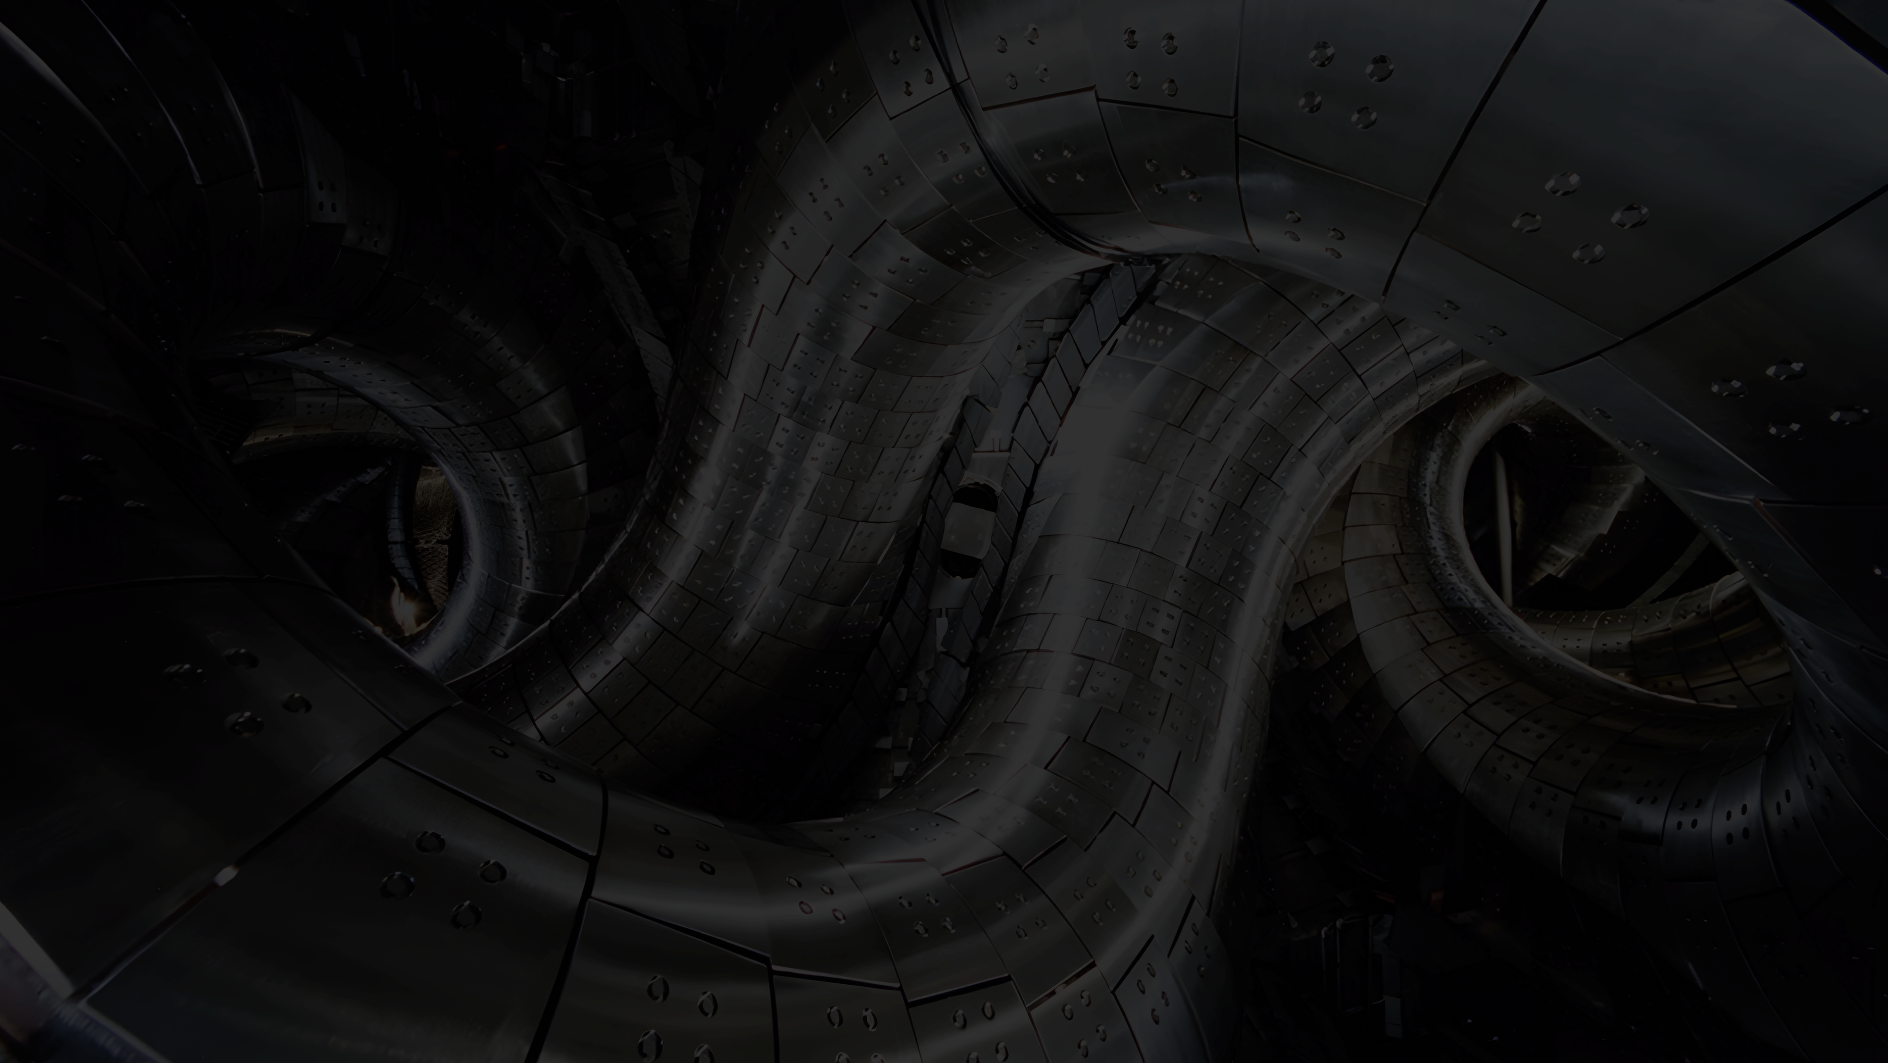
\includegraphics[width=\paperwidth,height=\paperheight]{background.png}%
}



\begin{document}
\color{LightGrey}
\begin{frame}{}
\color{LightGrey}
\maketitle
\end{frame}


% Local background must be enclosed by curly braces for grouping.
{
\begin{frame}{Inhalt}
\begin{itemize}
    \color{LightGrey}
\item Grundlagen der Kernfusion
\item Geschichte der Kernfusion
\item Stellare Kernfusion
\item Kernfusion zur Energiegewinnung
\end{itemize}
\end{frame}
}

{
\begin{frame}{Grundlagen der Kernfusion}
\begin{itemize}
    \color{LightGrey}
\item Verschmelzen von Atomkernen
\item Kerne müssen Coulombbarriere überwinden / durchtunneln   
\item Sowohl exotherme als auch endotherme Fusionsreaktionen
\item Exothermität / Endothermität durch Massendefekt zu erklären
\end{itemize}
\end{frame}
}

{
\begin{frame}{Geschichte der Kernfusion}
\begin{itemize}
    \color{LightGrey}
\item 1917, Lange vor Kernspaltung entdeckt
\item 1920 als Energiequelle von Sternen erkannt
\item 1952/53 erste auf Fusion bassierende Wasserstoffbombe
\item Seit Entwicklung der Fissions-Bombe Forschung an wirtschaftlicher Nutzung
\end{itemize}
\end{frame}
}

{
    \begin{frame}{Stellare Kernfusion}
        \begin{itemize}
            \color{LightGrey}
            \item Kleinere Sterne - Proton-Proton-Reaktion
            \item Größere Sterne - Bethe-Weizsäcker-Zyklus
            \item Entstehung von Kernen bis A = 60/70
        \end{itemize}
    \end{frame}
}


{
\begin{frame}{Proton-Proton-Reaktion}
    \begin{columns}
        \begin{column}{0.5\textwidth}
            \begin{itemize}
                \color{LightGrey}
                \item asdasdasda
            \end{itemize}
        \end{column}

        \begin{column}{0.5\textwidth}
            \begin{itemize}
                \color{LightGrey}
                \item Hauptreaktion der Sonne
                \item ca. \num{1.4e10} Jahre bis Start reaktion pro Proton
                \item + \num{26.196} MeV
            \end{itemize}
        \end{column}
    \end{columns}
    

\end{frame}
}

{
\begin{frame}{Bethe-Weizsäcker-Zyklus}

\begin{itemize}
\color{LightGrey}
\item
\begin{math}
    {\displaystyle \mathrm {_{\ 6}^{12}C+_{1}^{1}H\to _{\ 7}^{13}N+\gamma+1,96 \ MeV}}
\end{math}

\item 
\begin{math}
    {\displaystyle \mathrm {_{\ 7}^{13}N \to _{\ 6}^{13}C+ {e}^{+} + \nu_{e}+1,37 \ MeV }}
\end{math}

\item \begin{math}
    {\displaystyle \mathrm {_{\ 7}^{13}N \to _{\ 6}^{13}C+ {e}^{+} + \nu_{e}+1,37 \ MeV }}
\end{math}

\item
\begin{math}
    {\displaystyle \mathrm {_{\ 6}^{12}C+_{1}^{1}H\to _{\ 7}^{14}N+\gamma+7,54 \ MeV}}
\end{math}

\item
\begin{math}
    {\displaystyle \mathrm {_{\ 7}^{14}N+_{1}^{1}H\to _{\ 8}^{15}N+\gamma+7,35 \ MeV}}
\end{math}

\item
\begin{math}
    {\displaystyle \mathrm {_{\ 8}^{15}O \to _{\ 7}^{15}N+{e}^{+} + \nu_{e}+1,73 \ MeV}}
\end{math}

\item
\begin{math}
    {\displaystyle \mathrm {_{\ 7}^{15}N+_{1}^{1}H \to _{\ 6}^{12}C+_{2}^{4}He+4,96 \ MeV}}
\end{math}

\end{itemize}





\end{frame}
}

{
\begin{frame}{Quellen}
\begin{itemize}
    \color{LightGrey}
\item https://www.fusion.kit.edu/downloads/Kernfusion.pdf
\item https://de.wikipedia.org/wiki/Kernfusion
\end{itemize}
\end{frame}
}

\end{document}